\section{Motivação}

\begin{frame}{Motivação}
    Crescimento no número de aplicações de algoritmos de processamento de áudio.
    \vspace{0.5cm}

    \begin{itemize}
        \item Detecção e reconhecimento de voz\begin{itemize}
            \item Smartphones
            \item Automação residencial
            \item Comunicação online
        \end{itemize}
        \item Cancelamento de eco 
        \item Separação de fontes
    \end{itemize}
\end{frame}

\begin{frame}{Deep Learning}
    Aumento no número de artigos que envolvem \textit{deep learning} publicados em grandes conferências.
    \vspace{0.5cm}

    \begin{figure} 
        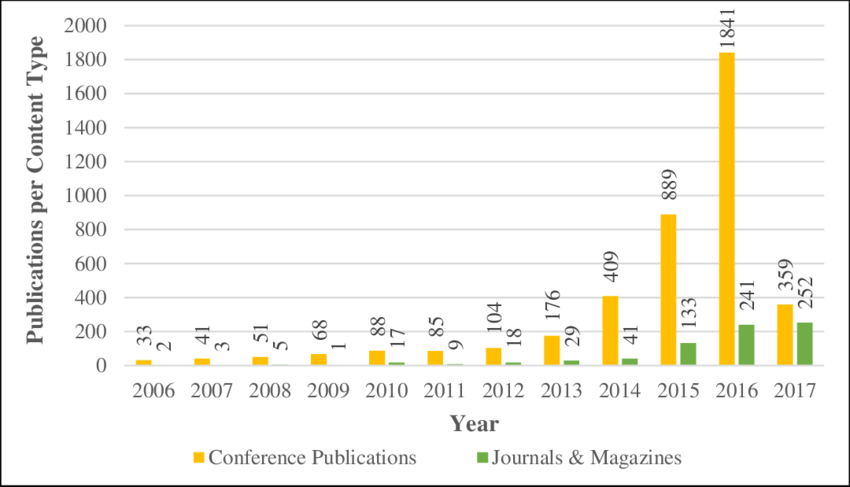
\includegraphics[scale=0.25]{pub_DL_IEEE.png}
        \label{fig:pub_DL_IEEE}
    \end{figure}
\end{frame}

\begin{frame}{Amostra de Voz em Campo Distante (AVCD)}
    Sinal de voz anecóico que é corrompido pela reverberação do ambiente fechado e ruído.
    \vspace{0.5cm}

    \begin{figure}
        \begin{subfigure}{.4\textwidth}
            \centering
            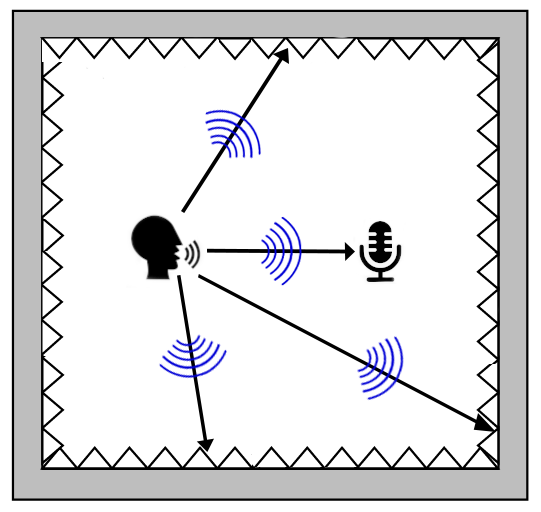
\includegraphics[scale=0.2]{camara_anecoica.png}
            \caption{Sala anecóica}    
        \end{subfigure}
        \begin{subfigure}{.4\textwidth}
            \centering
            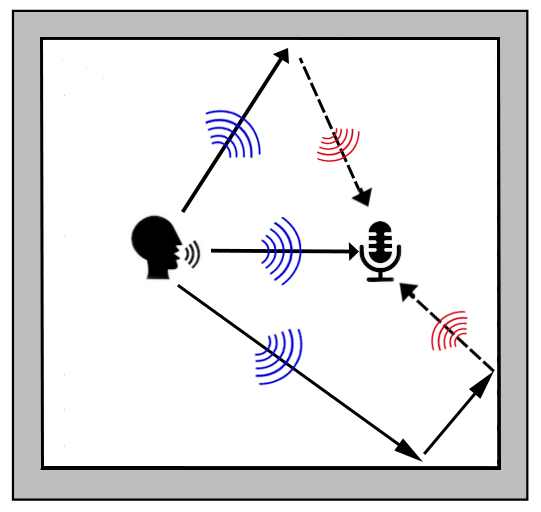
\includegraphics[scale=0.2]{camara_reverb.png}
            \caption{Sala reverberante}    
        \end{subfigure}
        \label{fig:Rooms}
    \end{figure}
\end{frame}

\begin{frame}{Amostra de Voz em Campo Distante (AVCD)}
    \begin{equation*} \label{eqn:model}
        Y(t) = s(t) \ast h(t) + n(t)
    \end{equation*}
    \vspace{0.5cm}

    $Y(t) \rightarrow$  AVCD \\
    $s(t) \rightarrow$  Amostra de Voz Anecóica \\
    $h(t) \rightarrow$  Resposta ao Impulso de Sala (RIR) \\
    $n(t) \rightarrow$  Sinal de Ruído \\
    
\end{frame}

\begin{frame}{Resposta ao Impulso de Sala (RIR)}
    Representa um modelo acústico de um ambiente para um par fonte/receptor.
    \vspace{0.1cm}

    \begin{itemize}
        \item Razão Direto-Reverberante (DRR)
        \item Tempo de Reverberação (T60)
    \end{itemize}

    \begin{figure} 
        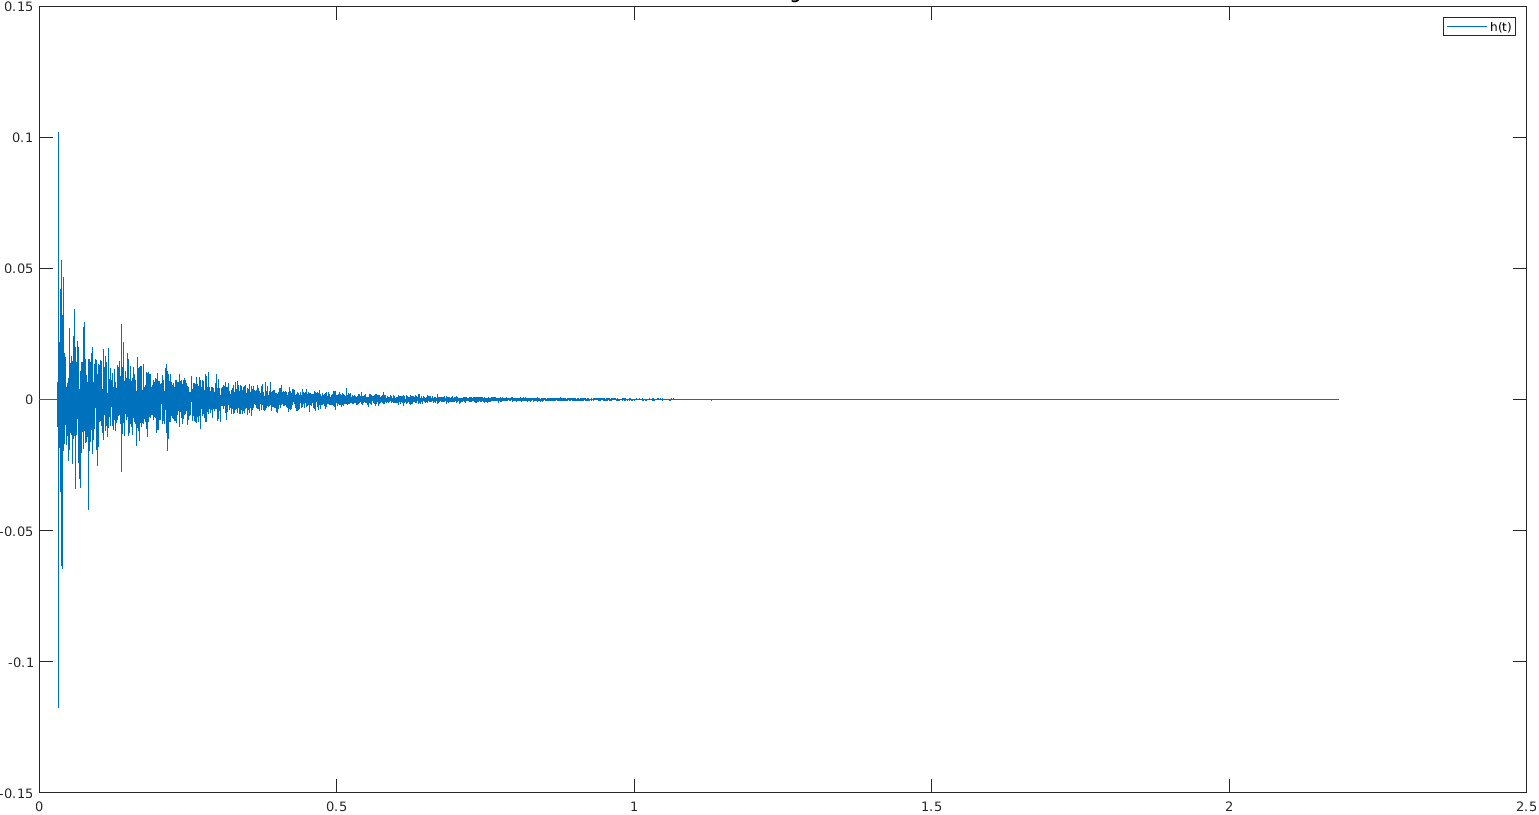
\includegraphics[scale=0.14]{rir-example.png}
        \caption{$DRR = -4,5$ dB / $T60 = 1,38$ s}
        \label{fig:rir-example}
    \end{figure}
\end{frame}

\begin{frame}{Desafios}
    \begin{itemize}
        \item Baixa quantidade e variedade de bases de dados contendo RIRs anotadas para treinamento de redes de \textit{deep learning}.
        \item Dificuldade para realizar gravações de RIRs (equipamentos especializados, variedade de ambientes, etc.)
    \end{itemize}
    \vspace{0.5cm}

    \begin{figure}
        \begin{subfigure}{.45\textwidth}
            \centering
            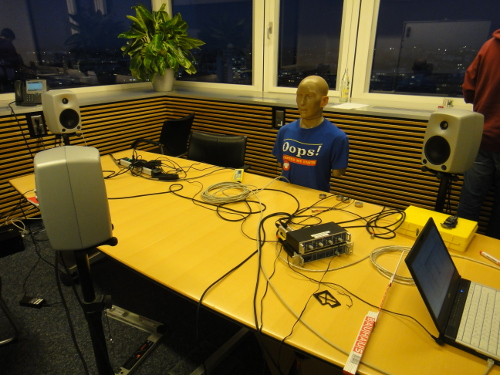
\includegraphics[scale=0.25]{recording.jpg}
        \end{subfigure}
        \begin{subfigure}{.45\textwidth}
            \centering
            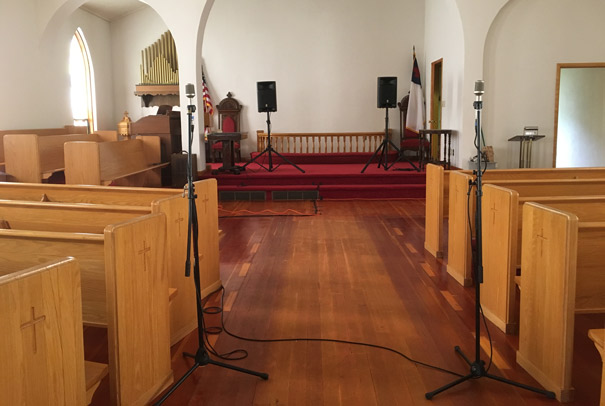
\includegraphics[scale=0.25]{recording3.jpg}
        \end{subfigure}
        \label{fig:recording}
    \end{figure}
\end{frame}